\documentclass[12pt]{article}
\usepackage[utf8]{inputenc}
\usepackage{amsmath}
\usepackage{graphicx}
\usepackage{float}
\usepackage[margin=1in]{geometry}
\usepackage{lineno}
\setlength{\parindent}{2em}
\setlength{\parskip}{1em}
\renewcommand{\baselinestretch}{1.2}
\newcommand\dbyd[2]{\frac{\mathrm d{#1}}{\mathrm d{#2}}}
\newcommand\dsided[2]{{\mathrm d{#1}}/{\mathrm d{#2}}}
\newcommand{\R}{\mathcal{R}}
\title{Intensional infect proportion of newborn, with disease induced mortality rate}
\usepackage{color}
\newcommand{\david}[1]{\textcolor{blue}{$\langle${\slshape{\bfseries David:} #1 }$\rangle$}}
\usepackage[colorlinks=true,linkcolor=blue]{hyperref}
\newcommand{\pmV}{p_{V}}
\newcommand{\pmI}{p_{I}}

\begin{document}
\linenumbers
\maketitle

\section{Motivation}

Previous analysis showed no obvious advantage for intentional infection. But those are the cases where we ignored disease induced mortality. In reality, if we are taking smallpox for example, past researches have determined the mortality rate to be 30 percent for normally infected cases, but only 1 percent for variolated cases. Thus, it is possible that intentional infection has a positive effect on disease control.

\section{Introduction}

Again, we consider two intentional infect strategies. One is to intentional infect newborns and the other is to intentional infect susceptible. In this document, we discuss the first strategy only.

\section{System of differential equations}
Since we have to consider disease induced mortality rate, we need to adjust our model by adding extra terms representing mortality rate.

The following assumptions are used:

\begin{itemize}
\item Birth and natural death rate are the same.
\item The latent period is short enough to be ignored.
\item All susceptible individuals are equally likely to be infected, and all infected individuals are equally infectious.
\end{itemize}

\begin{equation}\label{1}
\begin{split}
\dbyd{S}{t}&=\mu(1-p)- \beta S(V+I)-\mu S \,,\\
\dbyd{V}{t}&=\beta SV+\mu p-\gamma V -\mu V\,,\\
\dbyd{I}{t}&=\beta SI-\gamma I -\mu I\,,\\
\dbyd{M}{t}&=\pmV\gamma V+\pmI\gamma I\,,\\
\dbyd{R}{t}&=(1-\pmV)\gamma V+(1-\pmI)\gamma I-\mu R\,,
\end{split}
\end{equation}

Here, $\beta$ is the transmission rate, $\gamma$ is the recovery rate,
$\mu$ is the \emph{per capita} rate of birth and death, $p$ is the
proportion of newborns that are intentionally infected.

We non-dimensionalize \autoref{1} by scaling time, by
\begin{equation}
\tau=(\gamma+\mu)t \,,
\end{equation}

As the result, we obtain,
\david{Do not use hard-coded specific values of case fatality
  proportions.  Use symbols. $\pmV$, $\pmI$ for ``probability of
  mortality in $V$ or $I$ classes respectively}
\begin{subequations}\label{eq:base_ODE}
\begin{align}
\dbyd{S}{\tau}&=\epsilon(1-p)- \R_0 S(V+I)-\epsilon S\,, \label{eq:S_by_tau}\\
\dbyd{V}{\tau}&=\R_0 SV+\epsilon p-V\,, \label{eq:V_by_tau}\\
\dbyd{I}{\tau}&=\R_0 SI-I\,, \label{eq:I_by_tau}\\
\dbyd{M}{\tau}&=\pmV(1-\epsilon) V+\pmI(1-\epsilon) I\,,\\
\dbyd{R}{\tau}&=(1-\pmV)(1-\epsilon) V+(1-\pmI)(1-\epsilon) I-\epsilon R\,,
\end{align}
\end{subequations}

where $\epsilon=\frac{\mu}{\gamma+\mu}$, $\R_0=\frac{\beta}{\gamma+\mu}$.

\section{Equilibria}

To solve for all equilibria, we let equations \autoref{eq:S_by_tau}, \autoref{eq:V_by_tau} and \autoref{eq:I_by_tau} equal to 0, we solve solutions.

First by letting \autoref{eq:I_by_tau} equal to 0, we have either $S=\frac{1}{\R_0}$, $I=0$ or both. For the case where $S=\frac{1}{\R_0}$, \autoref{eq:V_by_tau} returns,
\begin{equation}
\dbyd{V}{\tau}=\epsilon p =0\,,
\end{equation}

Which has no solution if $p\neq 0$, and since we consider various possibilities where $p\neq 0$, we conclude that $S\neq\frac{1}{\R_0}$. Therefore, $I=0$.

Equipped with the above condition, we now solve the other two equations and the only solution we acquire is
\begin{subequations}
\begin{align}
\hat{S}&= \frac{1}{\R_0}-\frac{2p}{(\R_0 -1)+ \sqrt{(\R_0-1)^2+4\R_0
         p}}\,, \label{eq:Shat}\\
\hat{V}&= \frac{\epsilon(\R_0 -1)+ \epsilon \sqrt{(\R_0-1)^2+4\R_0 p}}{2\R_0}\,, \label{eq:Vhat}\\
\hat{I}&=0\,, \label{eq:Ihat}
\end{align}
\end{subequations}

At this equilibrium, since the infected population is non-zero, this is not a disease free equilibrium. It follows that the only equilibrium we found is an endemic equilibrium, and disease free equilibrium does not exist for this model.

\section{Stability of Endemic Equilibrium}

Stability analysis rely on Jacobian Matrix,
\begin{equation}
\mathcal{J} =
\begin{bmatrix}
    \ -\R_0 (V+I)-\epsilon       & -\R_0 S     &-\R_0 S\\
    \ \R_0 V       & \R_0 S-1    &0\\
    \ \R_0 I       &0     &\R_0 S-1\\
\end{bmatrix}\,.
\end{equation}

Eigenvalues of Jacobian are given as follow,
\begin{subequations}
\begin{align}
\lambda_1&=-1+\R_0 S \label{eq:lambda1}\\
\lambda_2&=\frac{-1+\R_0 S-\epsilon-\R_0 V-\sqrt{(-1+\R_0 S-\epsilon-\R_0 V)^2-4(\R_0+\epsilon-\R_0 S\epsilon)}}{2} \label{eq:lambda2}\\
\lambda_3&=\frac{-1+\R_0 S-\epsilon-\R_0 V+\sqrt{(-1+\R_0 S-\epsilon-\R_0 V)^2-4(\R_0+\epsilon-\R_0 S\epsilon)}}{2}\label{eq:lambda3}
\end{align}
\end{subequations}

By using \autoref{eq:Shat} and \autoref{eq:lambda1}, we obtain
\begin{equation}
-1+\R_0 S = - \frac{2p\R_0}{(\R_0 -1)+ \sqrt{(\R_0-1)^2+4\R_0 p}}<0
\end{equation}
Therefore, \david{eigenvalues must be written in $a+ib$ form, where
  $a,b$ are real.}
\david{You have not calculated the real parts of $\lambda_2$ and $\lambda_3$.}
\begin{equation}
\Re(\lambda_1) =-1+\R_0 S<0\,,
\end{equation}
To determine the real part of $\lambda_2$ and $\lambda_3$, we need to determine the sign of the quantity under the square root. 

By using \autoref{eq:Shat} again, we have
\begin{equation}
\R_0 S\epsilon<\epsilon\,,
\end{equation}

Therefore,
\begin{equation}
(\R_0+\epsilon-\R_0 S\epsilon)>\R_0 >0\,,
\end{equation}
which means, if the sign of the quantity under the square root is positive, we necessarily have
\begin{equation}
\sqrt{(-1+\R_0 S-\epsilon-\R_0 V)^2-4(\R_0+\epsilon-\R_0 S\epsilon)}<|(-1+\R_0 S-\epsilon-\R_0 V)|
\end{equation}
Therefore, $\Re(\lambda_2)<\Re(\lambda_3)<0$.

Certainly, if the sign of the quantity under the square root is negative,
\begin{equation}
\Re(\lambda_2)=\Re(\lambda_3)=-1+\R_0 S-\epsilon-\R_0 V<0
\end{equation}

We are able to conclude that EE is stable.
\section{Disease Free Equilibrium}
As mentioned above in section 4, disease free equilibrium does not exist for this model.
\section{Mortality rate at Endemic equilibrium}
When performing epidemic analysis, it is important to observe the mortality rate of the population, since this parameter is crucial to the severity of this disease. Here, we emphasize the mortality rate at EE.

By substituting the corresponding values at EE into equation (3d), we obtain,
\begin{equation}
\dbyd{M}{\tau}=\pmV(1-\epsilon)V=\frac{\pmV(1-\epsilon)\epsilon(\R_0 -1)+ \pmV(1-\epsilon)\epsilon \sqrt{(\R_0-1)^2+4\R_0 p}}{2\R_0}\,, \label{eq:dMdt}
\end{equation}
\autoref{eq:dMdt} reveals 3 important points. 

First, the mortality rate at the EE does increase as the proportion  $p$ of individuals who are intentionally infected is increased.  Nevertheless, the total mortality over any period will be less with intentional infection if the mortality rate form intentional infection is much lower than the disease-induced mortality rate from natural infection.  Consequently, it may be beneficial to have high $p$ during an initial outbreak, but once an equilibrium is reached, it is likely to be better to avoid intentional infection.  

Second, as expected, the probability $\pmV$ of mortality due to intentional infection plays a major role in the mortality rate at the EE. Meaning intentional infection is unwise if $\pmV$ is too high. 

Third, mortality rate $\dsided{M}{\tau}$ also increases as $\R_0$ increases. 

More specifically, we now consider the case of smallpox, i.e., the parameter values in \autoref{tab:params}.

\begin{table}[H]
\begin{center}
\caption{Model parameters and smallpox values.}
\label{tab:params}
\smallskip
\begin{tabular}{c|c|r}
{\bfseries Symbol} & {\bfseries Meaning} & {\bfseries Value} \\\hline
$\mu$ & Natural \emph{per capita} death rate & $\frac{1}{50*365}$ per day \\
$\gamma$ & Recovery rate & $\frac{1}{22}$ per day \\
$\R_0$ & Basic reproductive number & 4.5
\end{tabular}
\end{center}
\end{table}

Therefore, we can calculate $\epsilon=\frac{\mu}{\mu+\gamma}=0.0012$
\begin{equation}
\dbyd{M}{\tau}=0.00111111(0.00420902+\frac{100375\sqrt{12.25+18p}}{83466496})\,,
\end{equation}
\david{write that as $a + b\sqrt{c + d p}$, where $a,b,c,d$ are number given to three significant figures.}
So we plot $\dbyd{M}{\tau}$ as a function of $p$,
\begin{figure}[H]
  \centering
  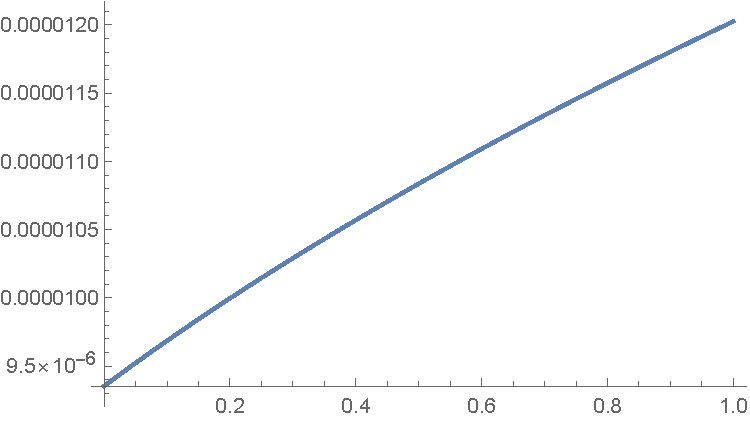
\includegraphics[width=1\textwidth]{Figures/Plot_dmdt_as_f_of_p.pdf}
  \caption{$\dbyd{M}{\tau}$ at EE as a function of $p$.}
\label{fig:dMdt}
\end{figure}

A major observation from this plot is, the magnitude of mortality rate at endemic equilibrium is far less than natural death rate. That is,
\begin{equation}
\left. \dbyd{M}{t}\right|_{\rm EE} \ll \epsilon 
\end{equation}
Consequently, once an equilbirium is reached, disease induced mortality will be negligible.  In \autoref{fig:dMdt} we demonstrate the total mortality counts as a function of time, using parameters from \autoref{tab:params}.
\begin{figure}[H]
  \centering
  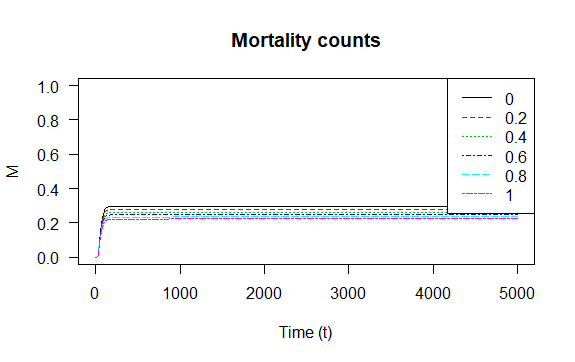
\includegraphics[width=0.7\textwidth]{Figures/Mortality_counts.png}
  \caption{$\dbyd{M}{\tau}$ at EE as a function of $p$.}
\label{fig:dMdt}
\end{figure}

Another plot to show the disadvantages of having a high proportion of intentional infection. This time, the variolation mortality is 20 percent instead of 1 percent.
\begin{figure}[H]
  \centering
  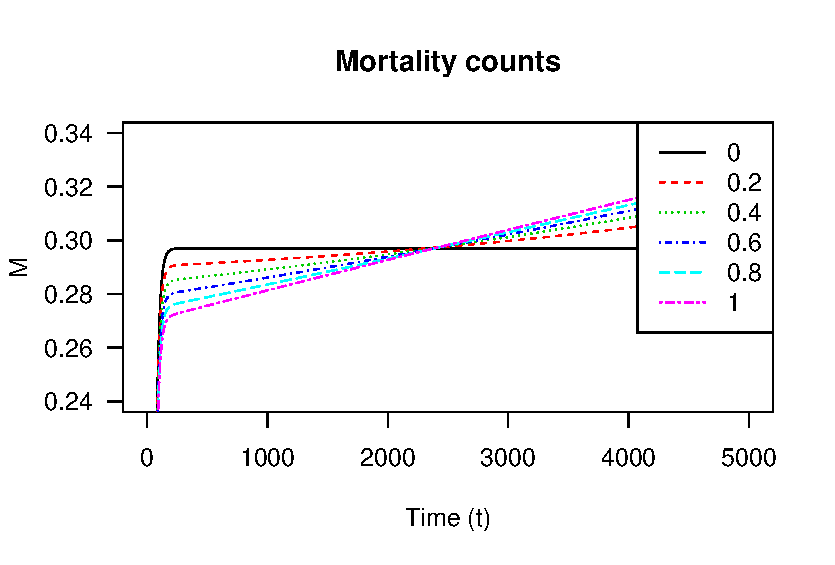
\includegraphics[width=0.9\textwidth]{Figures/Rplot.pdf}
  \caption{$\dbyd{M}{\tau}$ at EE as a function of $p$.}
\label{fig:dMdt}
\end{figure}
\section{Initial state being the Endemic Equilibrium of the model with no intentional infection}

We are interested in the scenario where intentional infection is only introduced after the population is in equilibrium, with no intentional infection.

We are interested in the time it takes to reach the new EE. Since the new equilibrium has $\hat{I}=0$, we define reaching equilibrium $I\leq 1\times 10^{-6}$ (one in a million).

Since a 1 percent variolation mortality rate would make the difference between different $p$ values insignificant, here we assume variolation mortality rate equal 20 percent, and that should help us observe the dynamics better.

by plotting, we obtain \autoref{lessthan0.000001}
\begin{figure}[H]
  \centering
  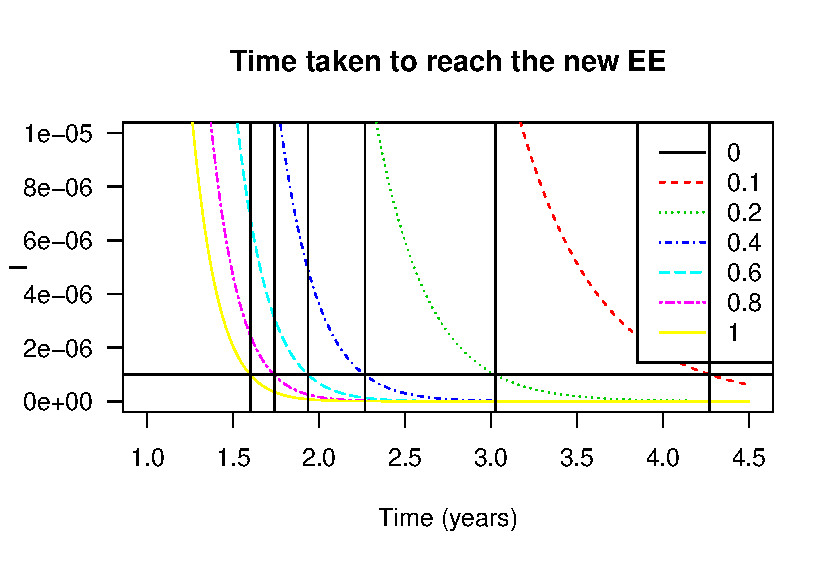
\includegraphics[width=1.1\textwidth]{Figures/I_less_than_0_000001.pdf}
  \caption{Determination of time taken to reach equilibrium}
\label{lessthan0.000001}
\end{figure}

We are also interested in the time it takes for intentional infection to take advantage over non-intentional infection, by comparing total mortality.

From previous analysis, we learned that $\dbyd{M}{\tau}$ decreases over time, and stabilizes at a constant rate when reaching the new EE. But at the new EE, $\dbyd{M}{\tau}$ is higher when $p$ is higher. 

\begin{figure}[H]
  \centering
  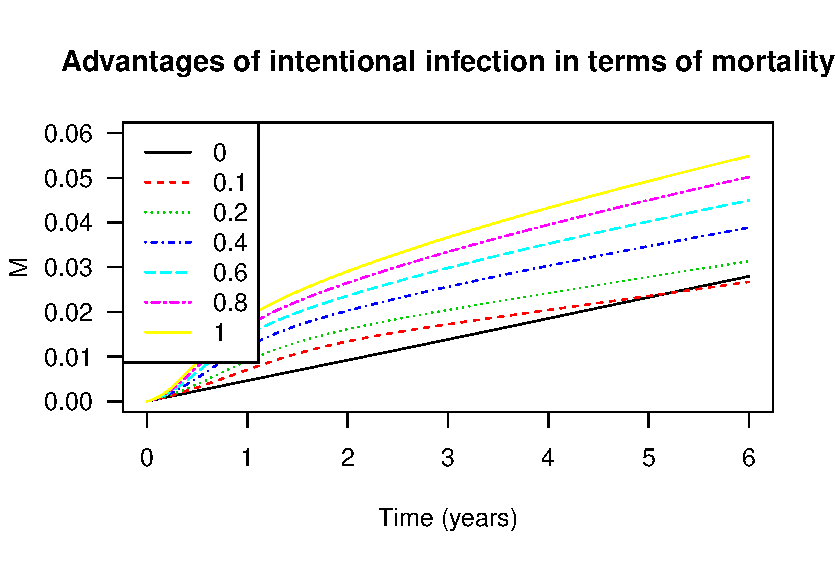
\includegraphics[width=1.1\textwidth]{Figures/dMdt.pdf}
  \caption{An illustration of intentional infection have advantages over non-intentional infection}
\label{lessthan0.000001}
\end{figure}

The graphs shows, at earlier times, intentional infections have steeper slopes than the black line, which is non-intentional infection. The slopes for intentional infection decreases over time, and eventually all of them have smaller slope than the black line.

\autoref{tab:times} summarize the times required to reach the new EE and time required to have advantages over non-intentional infection.

\begin{table}[H]
\begin{center}
\caption{Time required to reach equilibrium and have advantages over non-intentional infection}
\label{tab:times}
\smallskip
\begin{tabular}{c|c|r}
{\bfseries $p$} & {\bfseries Time to EE} & {\bfseries Time to have advantages} \\\hline
0.1 & 4.27 yrs & 5.20 yrs \\
0.2 & 3.03 yrs & 8.81 yrs \\
0.4 & 2.27 yrs & 17.45 yrs \\
0.6 & 1.94 yrs & 28.37 yrs \\
0.8 & 1.74 yrs & 42.43 yrs \\
1.0 & 1.60 yrs & 61.46 yrs
\end{tabular}
\end{center}
\end{table}

The table showed that as $p$ increases, the system reaches the new EE faster, but the time required to have advantages over non-intentional infection increase.

In fact, if $\pmV=0.01$, then the time required to have advantages over non-intentional infection is minimal, and the difference between different $p$ is also insignificant on a scale of years.

The observed "funny" fact is, the lower proportion we intentionally infect, the less time it takes to have advantages. But I believe the proportion cannot be too low, if it takes too long to reach the new EE, the slope may not decrease fast enough to be smaller than the slope of the black line, which may lead to increase of time required to have advantages.



\end{document}